%%%%%%%%%%%%%%%%%%%%%%%%%%%%%%%%%%%%%%%%%%%%%%%%%%%%%%%%%%%%%%%%%%%
\section{Étape 4: Sélection de la plateforme} \label{sec:methodo_step4}
%%%%%%%%%%%%%%%%%%%%%%%%%%%%%%%%%%%%%%%%%%%%%%%%%%%%%%%%%%%%%%%%%%%

Cette quatrième étape consiste à réaliser le choix de la plateforme la plus adaptée en prenant en compte différents critères.

%%%%%%%%%%%%%%%%%
\subsection{Motivations et objectifs}
%%%%%%%%%%%%%%%%%
    
    
    Les deux premières étapes ont permis de trouver et de caractériser de nouvelles plateformes. À l'aide de benchmark, plusieurs caractéristiques clefs des architectures ont pu être obtenues. Lors de l'étape 3, l'extraction et la modélisation des noyaux de calculs ont été faites. Il faut maintenant choisir quelle plateforme est adaptée à chaque noyau. Cependant, il ne faut pas tenir compte que de la performance, d'autres critères entrent en jeu et notamment le critère financier (voir \autoref{sec:methodo_step4}).
    L'objectif de cette étape est d'aider à la sélection des plateformes adaptées aux noyaux identifiés dans l'étape précédente.

    \begin{figure}
        \center
        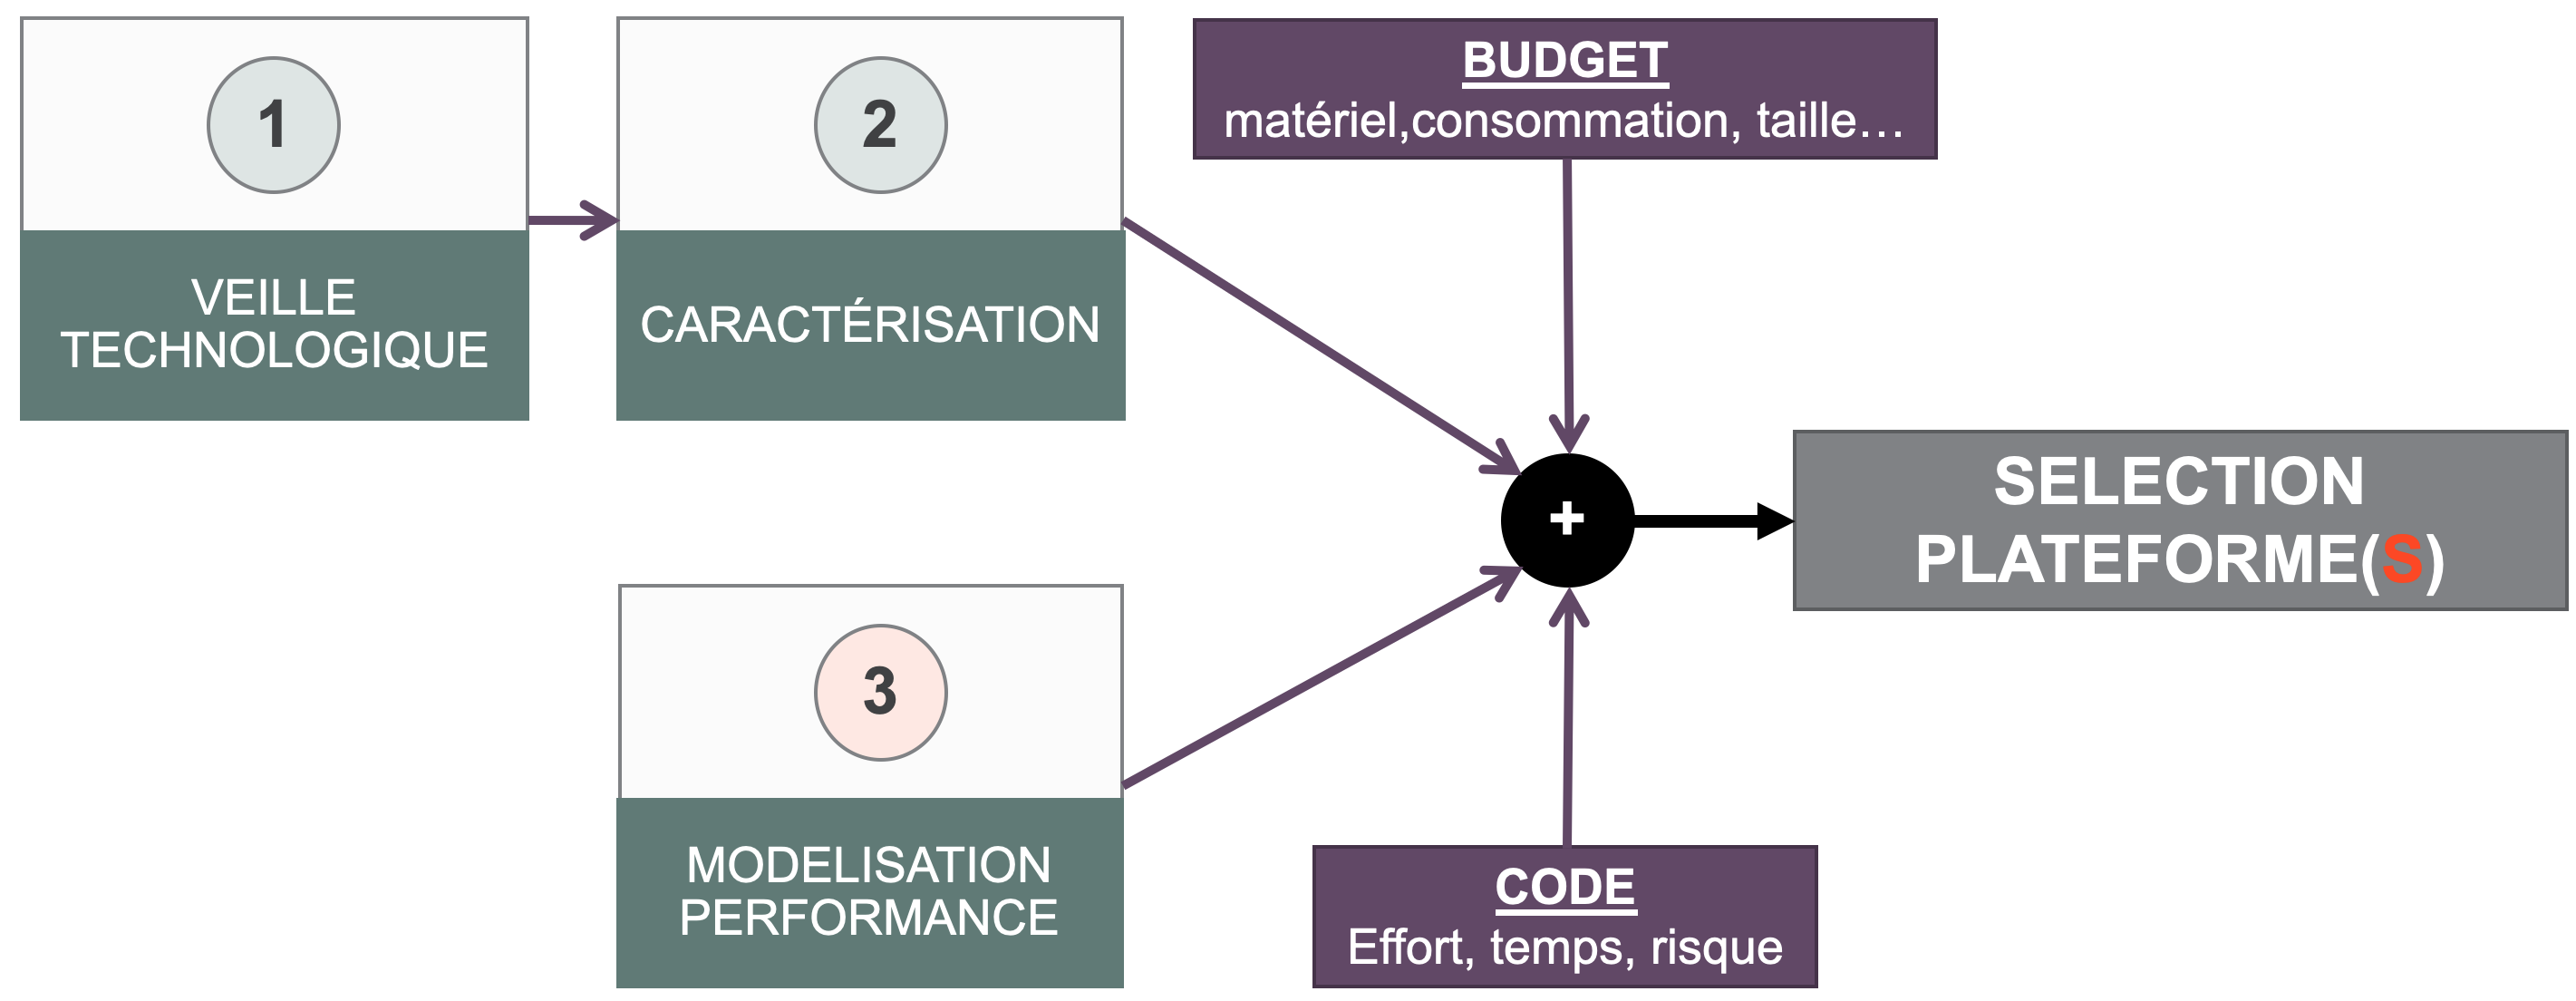
\includegraphics[width=14cm]{images/methodo_step4.png}
        \caption{\label{pic:methodo_step4}L'étape 4 consiste à choisir les plateformes adaptées aux différents noyaux en fonction de plusieurs critères.}
    \end{figure}



%%%%%%%%%%%%%%%%%
\subsection{Le coût}
%%%%%%%%%%%%%%%%%
    
    Le coût de l'architecture choisi est important, mais aussi celui de la solution globale. Beaucoup de paramètres entrent en jeu dans le calcul de prix total appelé coût total de possession ($\text{TCO}$). Il prend en compte tous les coûts engendrés par le centre de données durant son cycle de vie. Le budget pour la construction du premier centre exascale européen est de 500 millions d'euros \cite{SergiGirona2018}.
    
    \subsubsection{Le prix du matériel} 
        Le  prix des accélérateurs et du matériel nécessaires à la construction du supercalculateur constituent une part significative dans le calcul du coût (\textbf{todo: une idée ?}). En fonction du prix de l'accélérateur, une solution moins performante pourra lui être préférée. Les cartes FPGA sont un bon exemple d'architectures très performante mais peu utilisées dans les supercalculateurs. Bien que la complexité de programmation y participe, le prix des cartes FPGA est une raison majeure de leur faible utilisation dans les plateformes modernes.
    
    \subsubsection{La consommation électrique}
        La majorité des centres de données ont des lignes électriques déjà construites permettant d’acheminer une quantité limitée de courant. La consommation électrique de la plateforme finale est devenue un critère très important dans le choix du matériel. La consommation des centres de données est un réel investissement qui doit être mesuré et anticipé lors de l'achat du matériel. Un supercalculateur consommant 10 Mwatt engendrera une facture plusieurs millions d'euros chaque année. Le prix de l'électricité et l'enveloppe énergétique disponible pour le calcul dépendent de la localisation du centre de données. La chaleur de la zone géographique de son installation impactant le refroidissement nécessaire. Ainsi en 2018, Microsoft a décidé de couler ses serveurs au fond de l'océan pour profiter d'un refroidissement gratuit \cite{ChristineHall2018}.
        
    \subsubsection{La taille du centre de données} 
        Souvent les centres de données sont déjà existants et la taille disponible pour la création d'un supercalculateur ou l'ajout de nouveaux serveurs est une contrainte forte. Certaines solutions prenant plus ou moins de place pour être installées, le ratio $\frac{flop}{m^2}$ peut alors être calculé pour évaluer la densité des serveurs pour s'adapter aux contraintes du lieu. Si le bâtiment doit être construit pour accueillir le supercalculateur, son coût doit entrer dans le calcul de la solution finale.




%%%%%%%%%%%%%%%%%
\subsection{La performance}
%%%%%%%%%%%%%%% \cite{Rodero2012}%%
    
    \subsubsection{Performance du noyau}
        Le choix de l'accélérateur prend en considération la performance qu'aura l'application lorsque le noyau y sera porté. Les étapes 1 et 2 ont permis d'établir les performances d'une architecture. L'étape 3 à elle permis de modéliser les performances d'un noyau en fonction de la performance de la bande passante passante en calculant $\text{TEMPS}_{optimal}$, le temps optimal pour exécuter ce noyau sur l'architecture considérée.
    
    \subsubsection{Efficacité énergétique}
        En comparant son intensité opérationnelle  $\text{OI}_{noyau}$ et l'équilibre arithmétique de la plateforme $\text{EQUILIBRE}_{plateforme}$ il est possible d'estimer la pertinence d'un accélérateur pour un noyau. Des valeurs proches indiquent que l'architecture ciblée est adaptée au code étudié et que l'accélérateur choisi aura un meilleur rendement énergétique. Un code faisant peu de calculs flottants ne nécessitera pas l'utilisation de coeurs complexes réalisant plusieurs dizaines de flop par cycle. Bien que non utilisés, ces composants impactent le prix de la solution, mais aussi sa consommation électrique. Une grande part des centres de données consomme aujourd'hui la totalité de l'électricité disponible. Ces supercalculateurs doivent alors se tourner vers des solutions plus efficaces énergiquement ou le \textit{cloud} \cite{Rodero2012}.
        
    
    \subsubsection{Difficulté du portage}
        Le code de l'application  et les transformations nécessaires doivent être pris en compte, car il peut avoir un impact sur les performances ou sur le coût. Le travail de portage de l'application sur une nouvelle architecture doit être anticipé. Suivant l'architecture choisie, il faudra peut-être coder l'application avec un nouveau langage, utiliser de nouvelles librairies ou de nouveaux modèles de programmation. Le temps $\text{TEMPS}_{optimal}$, pour exécuter l'application considère que l'application utilise de façon optimale l'architecture. Cependant pour atteindre ces performances, le noyau peut nécessiter d'être optimisé et certaines peuvent être très difficiles à implémenter sur des codes existants. Certaines optimisations nécessitent une réelle expertise du domaine et du matériel envisagé. Lorsqu'une optimisation est choisie d'être implémentée le risque de ne pas parvenir à obtenir les performances espérées doit lui aussi être mesuré. Il peut arriver qu'une optimisation moins performante soit préférée, car la transformation du code est plus facile. Le temps et le nombre de programmeurs nécessaires à son implémentation entrent aussi en considération dans le prix de la solution.
    
    
    \subsubsection{Performance des applications }
        La performance du noyau a un impact financier, car s'il est exécuté plus rapidement, d'autres applications pourront alors accéder à la plateforme. Les clients de supercalculateurs ont généralement un budget fixe et de multiples applications à exécuter. Ils cherchent alors à optimiser l'utilisation des ressources informatiques par les différents codes. Bien que l'on considère de porter individuellement chaque noyau sur un accélérateur le plus adapté, il faut aussi prendre en considération le reste de l'application, mais aussi celle des autres utilisateurs. Si une seule des applications exécutées par l'utilisateur ne bénéficie des performances d'un accélérateur, il serait plus pertinent d'opter pour un accélérateur adapté au plus d'applications possible. 

                            